%\title{LaTeX Portrait Poster Template}
%%%%%%%%%%%%%%%%%%%%%%%%%%%%%%%%%%%%%%%%%
% a0poster Portrait Poster
% LaTeX Template
% Version 1.0 (22/06/13)
%
% The a0poster class was created by:
% Gerlinde Kettl and Matthias Weiser (tex@kettl.de)
% 
% This template has been downloaded from:
% http://www.LaTeXTemplates.com
%
% License:
% CC BY-NC-SA 3.0 (http://creativecommons.org/licenses/by-nc-sa/3.0/)
%
%%%%%%%%%%%%%%%%%%%%%%%%%%%%%%%%%%%%%%%%%

%----------------------------------------------------------------------------------------
%	PACKAGES AND OTHER DOCUMENT CONFIGURATIONS
%----------------------------------------------------------------------------------------

\documentclass[a0,portrait]{a0poster}

\usepackage{multicol} % This is so we can have multiple columns of text side-by-side
\usepackage{algorithm}
\usepackage{algorithmic}
\columnsep=100pt % This is the amount of white space between the columns in the poster
\columnseprule=3pt % This is the thickness of the black line between the columns in the poster

\usepackage[svgnames]{xcolor} % Specify colors by their 'svgnames', for a full list of all colors available see here: http://www.latextemplates.com/svgnames-colors

\usepackage{times} % Use the times font
%\usepackage{palatino} % Uncomment to use the Palatino font

\usepackage{graphicx} % Required for including images
\graphicspath{{figures/}} % Location of the graphics files
\usepackage{booktabs} % Top and bottom rules for table
\usepackage[font=small,labelfont=bf]{caption} % Required for specifying captions to tables and figures
\usepackage{amsfonts, amsmath, amsthm, amssymb} % For math fonts, symbols and environments
\usepackage{wrapfig} % Allows wrapping text around tables and figures
\newcommand{\bart}{\mbox{\tiny BART}}
\newcommand{\gp}{\mbox{\tiny GP}}


\begin{document}

%----------------------------------------------------------------------------------------
%	POSTER HEADER 
%----------------------------------------------------------------------------------------

% The header is divided into two boxes:
% The first is 75% wide and houses the title, subtitle, names, university/organization and contact information
% The second is 25% wide and houses a logo for your university/organization or a photo of you
% The widths of these boxes can be easily edited to accommodate your content as you see fit

\begin{minipage}[b]{0.75\linewidth}
\VeryHuge \color{NavyBlue} \textbf{Bayesian Additive Regression Trees for Bayesian Quadrature} \color{Black}\\ % Title
\huge 
	Ruya Kang, J\'er\^{o}me Liu, \textbf{Zhichao Shen}, Harrison Zhu, \textbf{Seth Flaxman}\\[0.5cm] % Author(s)
%\huge Imperial College London\\[0.4cm] % University/organization
\Large \texttt{s.flaxman@imperial.ac.uk} --- www.sethrf.com \\
\end{minipage}
%
\begin{minipage}[b]{0.25\linewidth}

\includegraphics[width=18cm]{icl}\ 
\end{minipage}

\vspace{-1cm} % A bit of extra whitespace between the header and poster content

%----------------------------------------------------------------------------------------

\begin{multicols}{3} % This is how many columns your poster will be broken into, a portrait poster is generally split into 2 columns

%----------------------------------------------------------------------------------------
%	ABSTRACT
%----------------------------------------------------------------------------------------

\color{Navy} % Navy color for the abstract

\section*{Overview}
	\begin{itemize}
		\item Bayesian Quadrature (BQ) can be used for problems with an integral at their heart. 
		\item We propose a new approach to BQ based on Bayesian Additive Regression Trees (BART). 
		\item BART is easy to tune, automatically handles a mixture of discrete and continuous variables, and has attractive theoretical results \cite{rockova2019theory,linero2018bayesian}. 
		\item BART-BQ outperforms Gaussian process-BQ and Monte Carlo integration for $d > 10$ and non-smooth functions.
		\item We propose Bayesian survey design with BART, as an effective alternative to simple random sample (Monte Carlo) and block random sampling designs.
	\end{itemize}
	
\color{Black} % Saddlrown color for the introduction


\section*{Bayesian Quadrature}
\begin{center}\vspace{1cm}
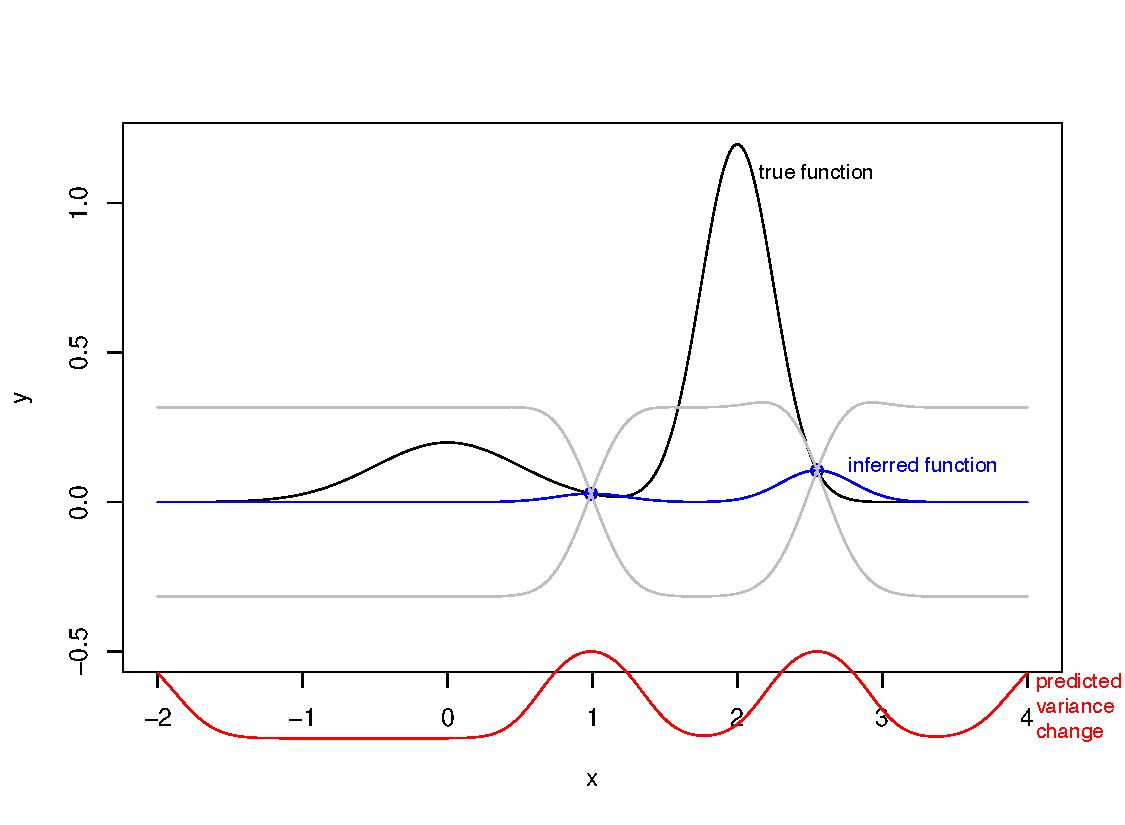
\includegraphics[width=1\linewidth]{illustration-sbq-3}
\end{center}
Given a function $f:\mathbb{R}^d \rightarrow \mathbb{R}$, build a probabilistic model for the integral:
\begin{equation}
	I_f =\int_{\mathbb{R}^d} f d\mu = \int_{\mathbb{R}^d} f(x) p(x) dx,
\label{eq:integral}
\end{equation}
	{\bf Standard approach.} Model using a GP: $f_{\gp} \sim \mathcal{GP}(\mu, k(\cdot,\cdot))$ 
\begin{align}
	\mbox{E}[I_f] &= \sum_{i=1}^n z^{\top} K^{-1} f_{\gp}(x_i) \\
	\mbox{Var}[I_f] &= \int \int k(x,x') p(x)p(x') dx dx' - z^{\top}K^{-1}z
\end{align}
	for $n$ observations $x_1, \ldots, x_n$ and $z_i = \int k(x,x_i) p(x) dx$

	Applications: uncertainty quantification \cite{oates2019bayesian}, probabilistic inference \cite{gunter2014sampling}, design of experiments/surveys?

%----------------------------------------------------------------------------------------
%	INTRODUCTION
%----------------------------------------------------------------------------------------

\section*{BART}
Given a $p$-dimensional input $x=(x_{1}, \ldots, x_{p})\in\mathbb{R}^p$ and its response $Y$, BART \cite{BART} aims to make inference on an underlying and unknown regression function
\begin{equation}
    Y = f(x) + \epsilon\text{, }\epsilon \sim N(0,\sigma^{2}),
\label{eq:underlying function}
\end{equation}

by estimating $f(x) = E(Y|x)$. For a BART model, for every posterior draw we have that for each tree $T$, with $b$ terminal nodes and a set of parameters $\Theta = \{\theta_1, \ldots, \theta_b\}$, with $\theta_i$ associated to the $i^{th}$ terminal node, denote,  $g(x; T, \Theta)$ as the step function which assigns each $\theta_i \in \Theta$ to $x$. Thus, a single tree BART model can be expressed as 
\begin{equation}
    E(Y|x) = g(x; T, \Theta).
\label{eq:single tree}
\end{equation}
Now define the sum-of-trees models as
\begin{equation}
    Y = \sum_{j = 1}^{m}g_j(x; T_j, \Theta_j) + \epsilon\text{, }\epsilon \sim N(0, \sigma^2),
\label{eq:single tree}
\end{equation}
where $m$ is the number of trees and $g_j(x; T_j, \Theta_j)$ is the function that assigns $\theta_{ij} \in \Theta_j$ to $x$.

For a fixed $m$ and a single draw from the posterior, the sum-of-trees model is determined by $(T_1, \Theta_1), (T_2, \Theta_2), \ldots, (T_m, \Theta_m)$ and $\sigma$.

\color{Black} % DarkSlateGray color for the rest of the content

\section*{Bayesian Quadrature (BQ) with BART}
Learn function $f_{\bart}$ and approximate Eq.~\eqref{eq:integral} with
\begin{equation}
	I_f \approx \int_{\mathbb{R}^d} f_{\bart} d\mu = \int_{\mathbb{R}^d} f_{\bart}(x)p(x)dx.
\label{eq:approx1}
\end{equation}

Since each tree is a step function, there are coefficients for each indicator function that we will call the ``value at the terminal node''. We denote the value of the $i^{th}$ terminal node of the $j^{th}$ posterior draw in the $k^{th}$ tree by $\theta_{i,j}^k$ . %Similarly, $p_{i,j}^k = \mu(\Omega_{i,j}^k)$ as discussed before in Eq~(\ref{eq:single tree approximation}). The details to obtain $p_{i,j}^k$ are included in subsection~\ref{p}.

Eq.~\eqref{eq:approx1} for the $j^{th}$ sum-of-trees:
\begin{align}
	I_f^{(j)} \approx \sum_{k=1}^{K}\sum_{i=1}^{b_{k,j}} \theta_{i,j}^k p_{i,j}^k,
\end{align}
where $b_{k,j}$ is the number of terminal nodes for tree $k$.

After fitting BART, we obtain $N$ draws from the posterior, and calculate $I_f^{(1)}, \ldots, I_f^{(N)}$. Any
posterior quantity of interest is available, e.g.:
\begin{equation}
	\mbox{E}[I_f|\mathcal{D}] \approx \frac{1}{N} \sum_{j=1}^{N} I_f^{(j)},
\end{equation}
\section*{Sequential BQ with BART}
Sequential design approach: randomly generate a set of candidates
$\mathcal{C} = \{c_1, \ldots, c_L\}\sim p(x)$. Find posterior variance of $f_{\bart}$ at $\mathcal{C}$. The point that we are least certain about (highest posterior variance) is the one that we will query next:
\begin{equation}
	c^* = \mbox{argmax}_{c \in C} \mbox{Var}[f_{\bart}(c) |\mathcal{D}]
	%\times p(c)],
	\label{eq:maxvariance}
\end{equation}
Having selected $c^*$ we query the true function $f$ to obtain $y_c^* = c^*$ and update our training set.

\begin{algorithm}[H]
  \caption{Sequential Design}
  \label{alg:SQ}
\begin{algorithmic}
  \STATE {\bfseries Input:}\\training set $\mathcal{D} = \{x_1, \ldots, x_n\}$, \\response $\mathcal{Y} = \{y_1, \ldots, y_n\}$, \\
  probability density function $p(x)$
  \FOR{$M$ iterations}
  \STATE obtain $N$ samples from the posterior distribution of the BART model with data $\mathcal{D}$ and $\mathcal{Y}$
  \STATE sample candidate set $\mathcal{C} = \{c_1, \ldots, c_L\}\sim p(x)$ 
  \STATE find $f_{\bart}^{(1)}(c), \ldots, f_{\bart}^{(N)}(c)$ for all $c\in\mathcal{C}$
  \STATE find $\,c^* = \mbox{argmax}_{c} \mbox{Var}[f_{\bart}(c)|\mathcal{D}]
	\label{eq:maxvar}$
  \STATE find response $y_c^* = f(c^*)$
  \STATE $\mathcal{D} \leftarrow \mathcal{D}\cup \{c^*\}$, $\mathcal{Y} \leftarrow \mathcal{Y}\cup \{y_c^*\}$
  \ENDFOR
\end{algorithmic}
\end{algorithm}
\label{Sequential Design}




\section*{Calculating terminal node probabilities}
\label{p}

Assume domain is $d$-dimensional hypercube and uniform probability measure $\mu$ over the inputs.
Figure 1 illustrates how we find the node probability on $d$-dimensional variables.
\begin{center}\vspace{1cm}
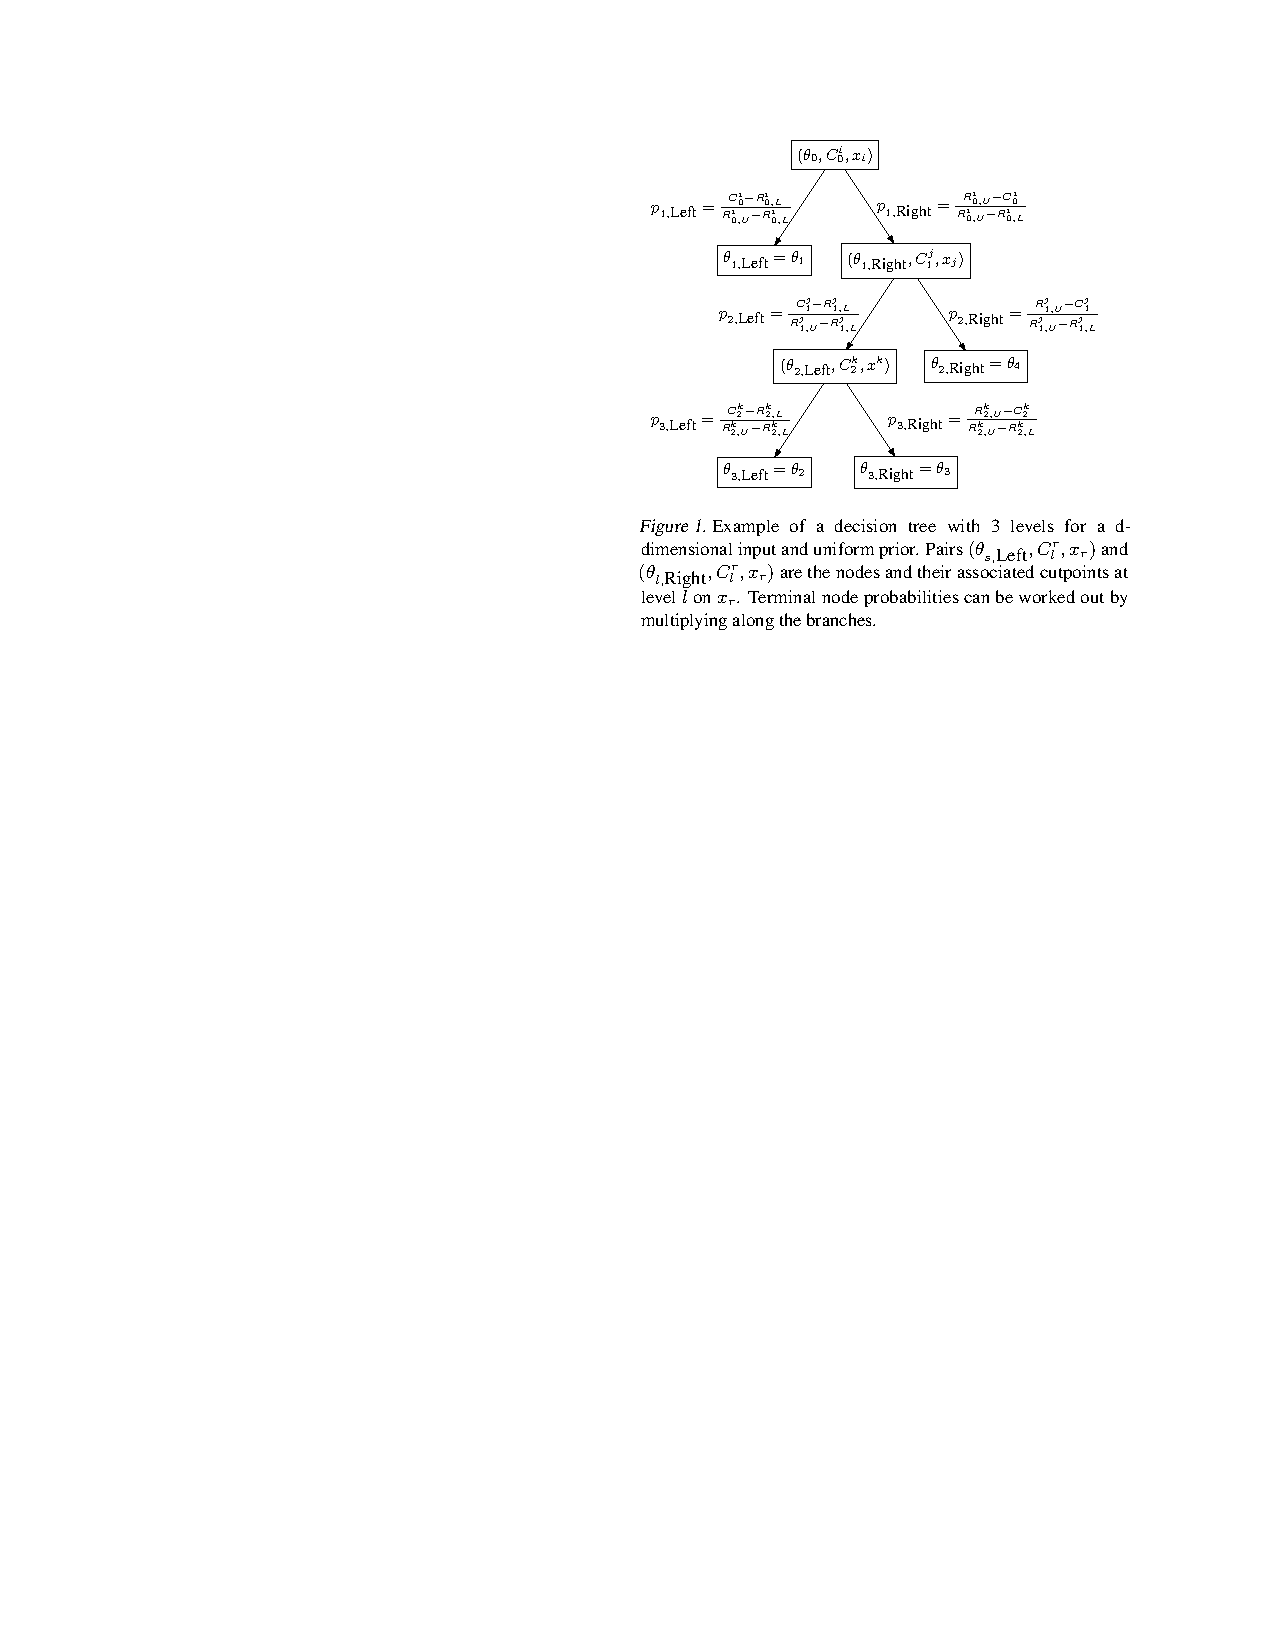
\includegraphics[width=.9\linewidth]{figure-1}
\end{center}

%For a tree in a posterior draw, the terminal node probability $p$ is obtained through multiplying the probability at leaf node $\theta_{l}$ at level $l$ of the tree along the branch. Suppose we have a $d$-dimensional uniform prior $p(x)$ in range $[0,1]^d$, and $x_r$ is the $r$th element in $x$, given the range $(R_{l,L}^r, R_{l,U}^r)$ of possible $x_r$ being allocated to the node $\theta_l$, and the cutpoint $C_l^r$ on $x_r$, the probability at the next left-branch node making decision on is
%\begin{equation}
%\label{eq:p(x)}
%    p_{l+1,\mbox{Left}} = \frac{C_l^r - R_{l,L}^r}{R_{l,U}^r - R_{l,L}^r}
%\end{equation}
%and the probability of the next right branch node is
%\begin{equation}
%    p_{l+1,\mbox{Right}} = 1-p_{l+1,\mbox{Left}} = \frac{R_{l,U}^r - C_l^r}{R_{l,U}^r - R_{l,L}^r}.
%%\end{equation}


%------------------------------------------------

\section*{Experimental Results: Genz benchmarks}

Standard benchmark set of multidimensional integrands proposed by Genz \cite{Genz}:
six families of functions with a set of parameters which can be varied to vary the level of difficulty of the integration problem. 

Compare rate of convergence for BART-BQ to Sequential Bayesian Quadrature with Gaussian processes (GP-BQ) \cite{ohagan1991bayes}.
and Monte Carlo (MC) sampling.

\begin{figure}[H]
\centering
\vspace*{-1.5in}
\includegraphics[width = 0.2\textwidth, angle = -90]{report/Figures/5/convergenceMean55Dimensions.eps}
\vspace*{-1in}
\caption{Convergence of the integral of the oscillatory Genz function of dimension 5 run with 500 epochs of sequential design. The actual integral is -0.08921 as indicated above.}
\label{fig:genz3}
\vspace*{-1mm}
\end{figure}
\begin{figure}[H]
\centering
\vspace*{-1.5in}
    \includegraphics[width = 0.2\textwidth, angle = -90]{report/Figures/3/convergenceMean320Dimensions.eps}
    \vspace*{-1in}
    \caption{Convergence of the integral of the discontinuous Genz function of dimension 20 run with 500 epochs of sequential design. The true integral value is 0.2816, as indicated above.}
\label{fig:genz3}
\vspace*{-1mm}
\end{figure}

\section*{Experimental Results: survey design}
2017 American Community Survey Public Use Microdata Sample (PUMS) from Wyoming, with demographic covariates. Goal: predict \texttt{income}. Goal: predict the average income of the the population as a whole and stratified by education level: high school education or above vs.~not. $N = $ 4,076. 

Assume we are given a set of samples $\mathcal{D} = \{x_i,y_i\}_{i=1}^n$, where $x_i$ is a demographic covariate vector and $y_i$ is a real-valued label. We have a further set of candidates $\mathcal{C} = \{c_1, \ldots, c_L\}$ with known covariates but unknown responses. The goal of our design is to sequentially select $M$ individuals.  In our application, $n = 50$ and $L = 4026$.

Fit BART to $\mathcal{D}$. This model can be used to provide posterior predictive distributions for each of the remaining individuals whose income information is missing. Denoting $f_P^j(x_i)$ as the prediction of individual $x_i$ given by the $k$th  draw from the posterior, we have the posterior estimated expected value of income 
\begin{equation}
\label{eq:mean}
    E[Y|\mathcal{D}] = \frac{1}{K}\sum_{k=1}^K\frac{1}{N}\sum_{i=1}^N f_P^j(x_i),
\end{equation}
where $N$ is the number of individuals with unknown income and $K$ is the number of posterior draws.

\begin{figure}[H]
    \centering
	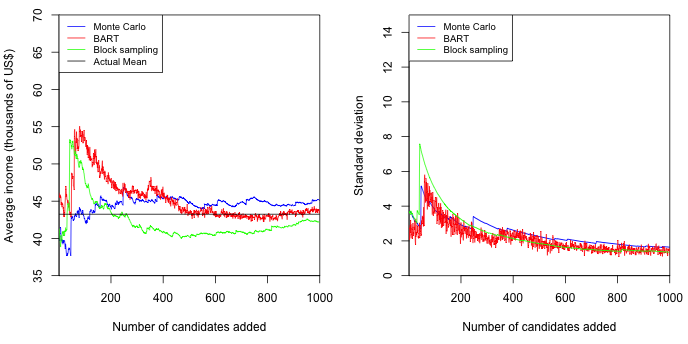
\includegraphics[width = 0.30\textwidth]{figures/population.png}
    \caption{Estimation (left) and standard error (right) of average total income (thousands of US\$) with different sampling methods.}

\end{figure}
\begin{figure}[H]
    \centering
	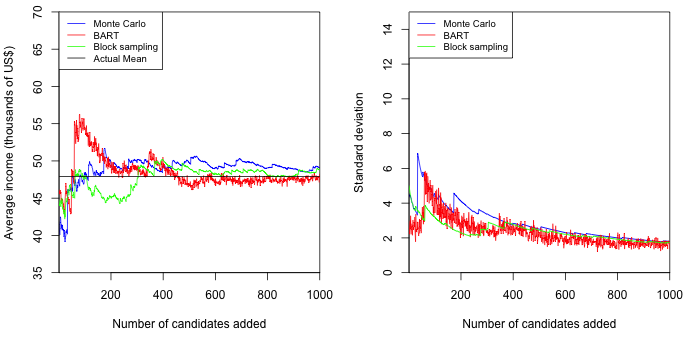
\includegraphics[width = 0.30\textwidth]{figures/high.png}
    \caption{Estimation (left) and standard error (right) of average total income (thousands of US\$) of population with education level beyond high school, given by different sampling methods.}


\end{figure}



%----------------------------------------------------------------------------------------
%	CONCLUSIONS
%----------------------------------------------------------------------------------------



%\nocite{*} % Print all references regardless of whether they were cited in the poster or not
\bibliographystyle{abbrv} % Plain referencing style
\bibliography{report/Writing/ref.bib} % Use the example bibliography file sample.bib

%----------------------------------------------------------------------------------------

\end{multicols}
\end{document}
